\documentclass{article}
\usepackage{amsmath,amssymb}
\usepackage{graphicx}
\newcommand{\E}{\mathop{\mathbb{E}}}
\begin{document}
\title{ \normalsize \textsc{}
		\\ [2.0cm]
		\LARGE \textbf{\uppercase{Exploring Human Motion Synthesis with Latent-Space GANs}
        }
		}
\date{\today}

\author{\textbf{Author} \\ 
		Vinitra Muralikrishnan}

{\let\newpage\relax\maketitle}
\tableofcontents
\newpage

\section{GANs}
GANs (Generative Adversarial Networks) are a class of ML models that consist of 2 neural networks -
a generator or a discriminator, that are trained simultaneously in a competitive setting.\\

\subsection{Components of GAN}
\begin{itemize}
\item Generator: Generator's job is to mimic real data. It takes a random noise vector and generates a sample
that resembles the target data distribution. Over time, it learns to genrerate samples tahta re more realistic.
\item Discriminator: It is a classifier that will classify between real data and fake data that is generated by the generator.
\item Training: The generator tries to fool the discriminator by generating better data and discriminator tries to become
better at distinguishing between real and fake. Both networks are trained in an adversarial manner. The loss function
of the generator is designed to maximize the chance of fooling the discriminator and the discriminator minimizes the classification
error betweeen real and fake data.
\item Challenges: Mode collapse, training instability and vanishing gradients. Mode collapse happens when generator produces
limited variations, failing to capture the full diversity of the real data (supposedly captured by mode).

\end{itemize}

\subsection{GAN training}
During the GAN training, the generator wants to fool the discriminator successfully and therefore the generator loss
would involve minimizing the log likelihood of discriminator being right. The discriminator on the other hand,
would work towards maximizing the log likelihood of discriminator being right.\\
$$V(G, D) = \E_{x \sim p_{data}} \mathop{log} D(x) + \E_{z \sim p} \mathop{log} (1 - D(G(z)))$$
In the above loss function, the generator loss would involve minimizing $\E_{z \sim p} \mathop{log} (1 - D(G(z)))$.
This is not a stable training process as the low quality samples wouldn't have large gradients with this equation.
The high quality samples would have large gradients, leading to bigger corrections in the generator and throw off the training.
Refer to the image below:\\
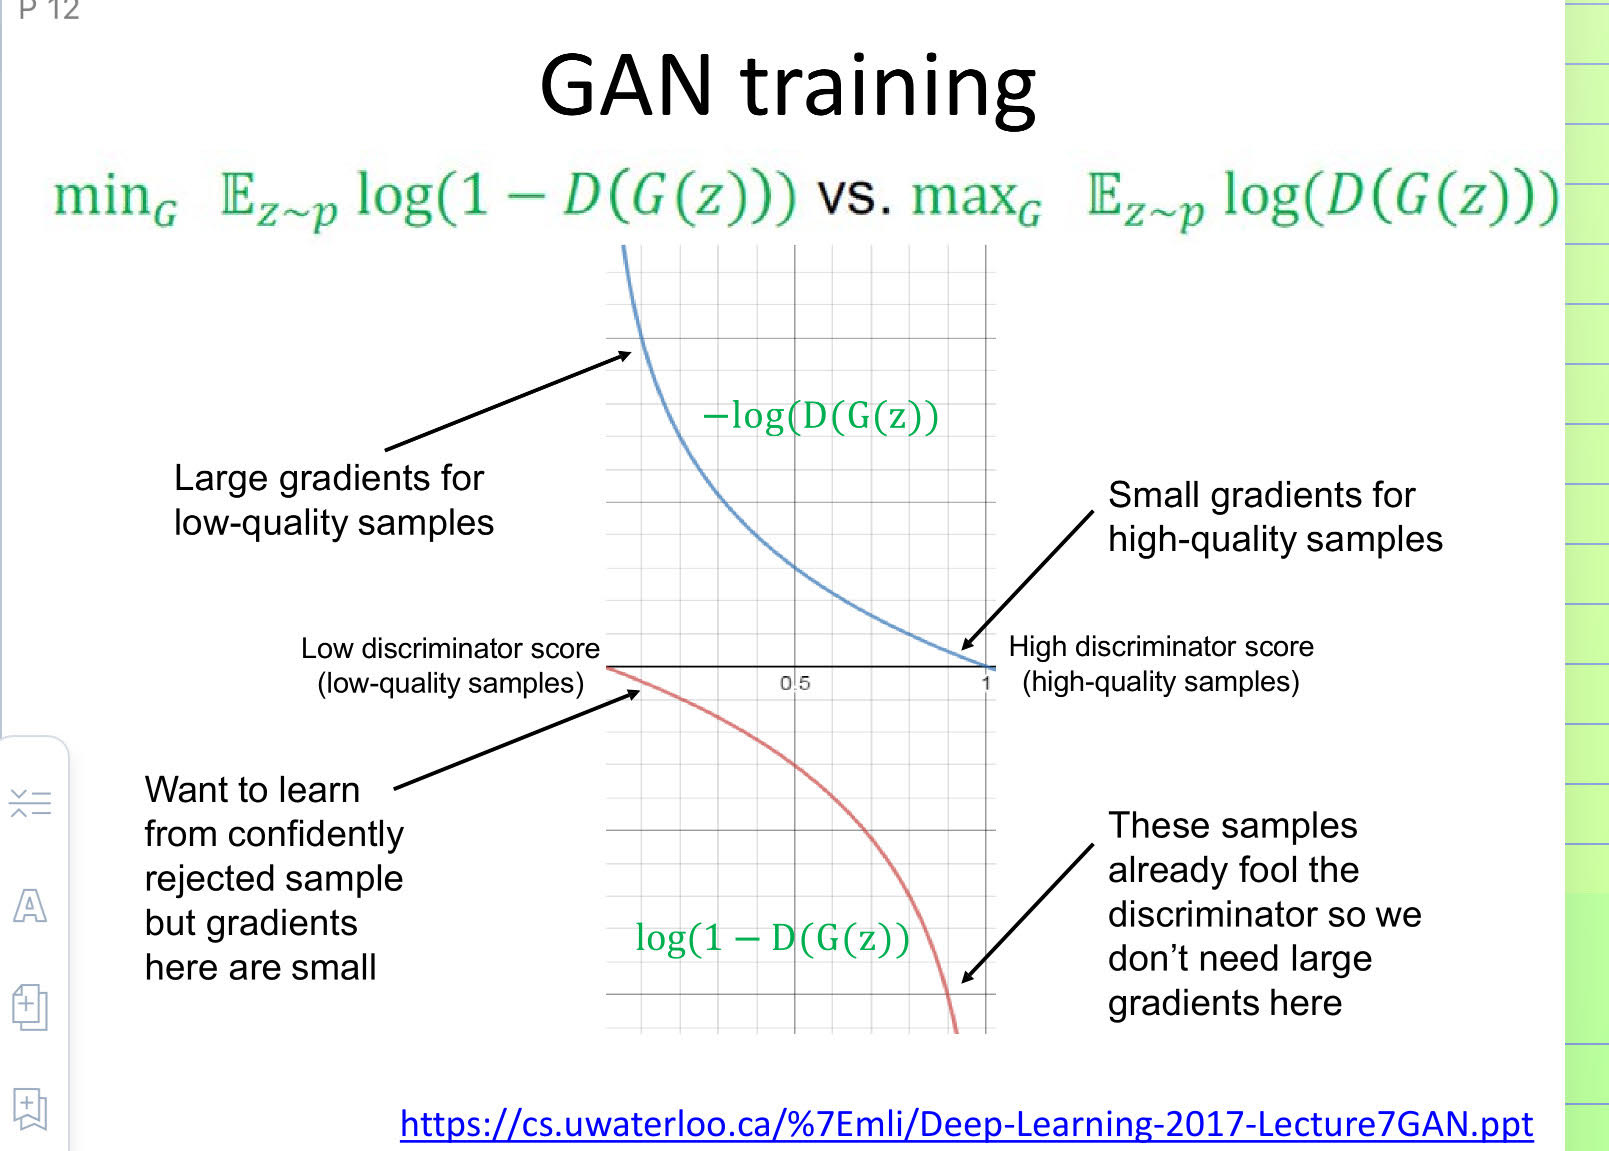
\includegraphics[width=5in]{./imgs/gan-training.jpg}\\\\
Therefore to correctly guide the generator, we instead choose to maximize the log likelihood of discriminator being wrong,
i.e $\E_{z \sim p} \mathop{log} (D(G(z)))$

\subsection{Variants}
\begin{itemize}
	\item DCGAN - uses convolutional layers instead of fully connected layers.
	\item WGAN - Uses wasserstein distance loss function instead of the original loss.
	\item StyleGAN: Allows more control over the generational process by separaing the high-level features and low-level features,
	resuling in impressive, fine-grained image generation.
	\item CycleGAN: Used for unpaired image-to-image translational tasks where images from one domain are transformed into another
	without needing paired samples.
	\item Condition GAN (cGAN): The generator and discriminator are conditioned on extra information such as text.
\end{itemize}
\subsection{StyleGAN}
Unlike traditional GANs where the generator takes a random noise vector as input, StyleGAN ues a style-based generator
and maps the random input to an intermediate latent space via a mapping network. This is done so the style can be controlled
better at different layers of the network. AdaIN (Adaptive Instance Normalization) is employed to apply styles at different layers of the generator.
This is done by adjusting mean and variance at each layer. This way the model can influce high-level features such as pose
and shape in early layers, fine-grained features such as textures and colors in later layers. This separation allows for precise
control over different aspects of the generated image. Next the StyleGAN generates image progressively from lower to higher 
resolutions. This ensures high fidelity outputs.\\
\textbf{Key takeaways:}\\
\begin{itemize}
	\item Separation of coarse and fine features
	\item Latent space manipulation
	\item Style mixing
\end{itemize}
\subsection{WGAN}
The classical GAN uses Jensen-Shannon Divergence. However, this method has issues while working with gradients that can
lead to unstable training. We therefore make use of Wasserstein distance to calculate the distance between 2 probability
distributions, which is given as follows:\\
$$\mathop{max}_{w \in W} \E_{x \sim P_r}[f_w(x)] - \E_{z \in p(z)}[f_w(g_\theta(z))]$$
In WGAN, the sigmoid is removed so the discriminator is more a critic than a discriminator. It gives high score
for realistic fake images and low score for bad fake data. The objective remains the same though. To ensure 1-Lipschitz
continuity of the disriminator score, gradient clipping was implemented initially. Without it, the WGAN suffered
from exploding gradients. This reduced the range of the critic score of WGAN critic. But gradient clipping didn't work
as optimally as expected. When weight clipping was sufficiently large, it led to longer training times as the critic
took a lot of time to adjust to the expected weights. When weight clipping was small, it led to vanishing gradients. For this,
the gradient penality was introduced. This involved adding a penalty term to the loss function that would penalize
the gradient norm if it deviated from 1. This method leads to smother training and better performance, since it allows the critic to have a more flexible
set of weights while ensuring the Lipschitz continuity.
\clearpage
\section{Variational Autoencoders}
They are also generative models that learn a probabilistic mapping from a latent space to a data distribution.
\subsection{Architecture}
It comprises of a encoder that maps input data to a latent space and outputs a mean and variance, parametrizing a
probability distribution. The VAE then samples from this distribution to a latent representation and introduces the 
stocahasticity that is key for generative tasks. The decoder then takes a sample from latent distribution and maps it back
to the origina space, reconstructing the input. VAE optimizes a reconstrctuion loss and a KL divergence loss, which ensures
that the latent space follows a known distribution (like a standard Gaussian). This regularization encourages,
smoother latent space repsentations that can be sampled from.
\section{About Motion Synthesis Problem}
\subsection{Metrics}
\begin{itemize}
	\item R-precision: Measures how well the generated motions match the expected action. Calculates the proportion of 
	relevant generated motions (correctly classified or corresponding to query) within the top k retrieved/generated samples.
	\item FID (Frechet Inception Distance): Evaluates the similarity between real and generated motion distributions. Computes distance
	between feature representations of real and generated data, capturing both mean and covariance of distributions.
	\item MM Distance (Multi-Modal distance): Measures how well the generated motions capture the multiple modes (variations)
	present in real data.
	\item Diversity: Quantifies the variability in the generated motion samples.
	\item M Modality: Evaluest the ability of a model to generate multiple distnct modes of motion condition on input.
\end{itemize}
\end{document}



